\chapter{Le triphasé}
\section{Notations - Conventions}
	
	\subsection{Conventions}
	\begin{wrapfigure}[10]{l}{3cm}
	\vspace{-5mm}
	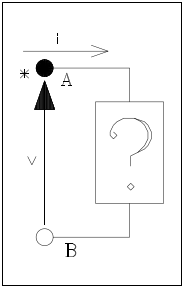
\includegraphics[scale=0.4]{ch1/image1.png}
	\captionof{figure}{ }
	\end{wrapfigure}
	La convention \textit{récepteur} sera celle utilisée : la puissance 
	sera positive lorsqu'elle sera absorbée par la machine. Pour une 
	source de tension $v$, c'est le contraire : le courant - défini par 
	les charges positives -sera dans le sens de la flèche.\\

	 L'astérisque 
	marque ainsi la borne d'entrée d'un dipôle ou un cercle plein.\\
	
	Dernière convention : la flèche de tension désigne la borne à 
	laquelle il faut appliquer une tension positive pour faire circuler 
	un courant positif.
	
	\subsection{Notations}
	\begin{tabular}{ll}
	$a = a(t)$ &: valeur instantanée\\
	$\underline{a}(t)$ &: valeur instantanée complexe ; vecteur tournant 
	dont la projection sur un axe de\\
	&\ \ \  référence fournit la valeur instantanée  
	d'une grandeur sinusoïdale de pulsation $\omega$ ; \\
	&\ \ \	$a(t) = \Re(
	\underline{a}(t))$\\
	$\underline{A} = A\angle\alpha$ &: nombre complexe de module $A$ et 
	d'argument $\alpha$.\\
	$A_M$ &: valeur de crête ou maximale dans le temps : $A_M = a \sqrt{2}$\\
	$\overline{A}$ &: vecteur spatial de module $A$\\
	$A^M$ &: valeur maximale d'une grandeur variant dans l'espace\\
	$i_{ab}$ &: courant circulant de $A$ vers $B$ ($A\rightarrow B$)\\
	$v_{ba} = v_a-v_b$ &: potentiel de $A$ par rapport à $B$ ($B \rightarrow A$)
	\end{tabular}

\section{Rappel de quelques notions relatives aux courants alternatifs}
	\subsection{Représentation des fonctions sinusoïdale du temps}
	Un telle grandeur, de pulsation $\omega$ est représentée par :
	\begin{equation}
	\begin{array}{lll}
	v &= V_M\cos(\omega t + \xi_v) & \text{où $V_M$ est la valeur de crete}\\
	 &= V\sqrt{2}\cos(\omega t + \xi_v) & \text{où $V$ est la valeur efficace}	
	\end{array}
	\end{equation}
	Ceci peut s'écrire 
	\begin{equation}
	\begin{array}{ll}
	v &= \Re (V\sqrt{2}\cos(\omega t + \xi_v) + jV\sqrt{2}\sin(\omega t + \xi_v))\\
	 &= \Re (V\sqrt{2}e^{j(\omega t + \xi_v})
	\end{array}
	\end{equation}
	La \textbf{valeur instantannée complexe} $\overline{v}$ est définie par \\
		\begin{wrapfigure}[12]{r}{5cm}
	\vspace{-15mm}
	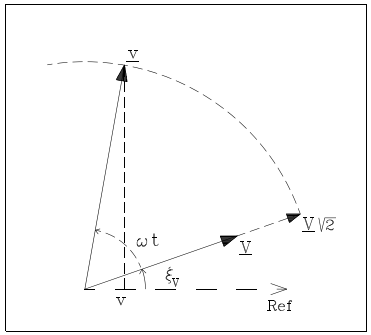
\includegraphics[scale=0.4]{ch1/image2.png}
	\captionof{figure}{ }
	\end{wrapfigure}
	\begin{equation}
	\begin{array}{ll}
	\overline{v} &= V \sqrt{2}e^{j(\omega t + \xi_V)}\\
	 &= V e^{j\xi_V}\sqrt{2}e^{j\omega t}
	\end{array}
	\end{equation}
	où le \textbf{phaseur} $\underline{V}$ est 
	\begin{equation}
	\underline{V} = Ve^{j\xi_V}
	\end{equation}
	Dans le plan de Gauss $\overline{V}$ a un module valant la valeur efficace 
	de la grandeur et un argument valant $\xi_V$, c'est un vecteur \textsc{fixe}.
	La valeur instantanée complexe $\underline{v}$ a un module $V\sqrt{2}$ et est 
	décalée de $V\sqrt{2}$ par rapport à $\overline{V}$ : c'est un vecteur 
	\textsc{tournant} (à $\omega$). On obtient la valeur instantanée en projetant 
	la valeur instantanée complexe sur l'axe réel : $v = \Re(\underline{v})$.\\
	
	Les déphasages entre grandeurs sont constants : on considère comme référence un 
	courant $\underline{I}$ et on définit l'argument de la tension par rapport à 
	celui-ci à l'aide de l'\textbf{angle de charge} $\varphi$.
	
	\begin{center}
	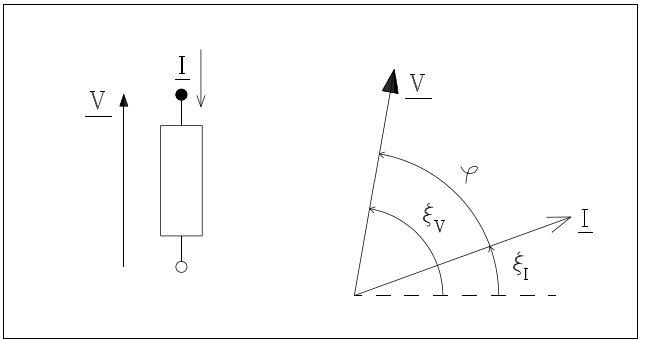
\includegraphics[scale=0.4]{ch1/image3.png}
	\captionof{figure}{ }
	\end{center}	
		
	Si l'on applique la tension $\underline{V} = V\angle \xi_V$ à une impédance 
	$\underline{Z} = R + jX = Z\angle \xi$, le courant vaut 
	\begin{equation}
	\underline{I} = \frac{\underline{V}}{\underline{Z}} = \frac{V}{Z}\angle 
	\xi_V-\xi
	\end{equation}
	On remarque avec l'argument du courant qu'une impédance inductive ($X>0, 
	\xi <0$) déphase le courant en arrière par rapport à la tension et l'inverse 
	pour une impédance capacitive.
	
	
	\subsection{Représentation de la puissance}
		\subsubsection{Puissance active}
		Cherchons à calculer la puissance de $A$ vers $B$ au point $X$. Nous 
		avons $v = V_M\cos(\omega t +\xi_V)$ et $i = I_M\cos(\omega t + \xi_I)$. 
		La valeur instantanée de la puissance vaut :
		\begin{equation}
		\begin{array}{ll}
		p &= v\ i\\
	      &= V_MI_M\cos(\omega t +\xi_V)\cos(\omega t +\xi_I)\\
	      &= \frac{V_MI_M}{2}(\cos(\xi_V-\xi_I) + \cos(2\omega t +\xi_V+\xi_I))\\
	      &= \underbrace{VI \cos\varphi}_{1} + \underbrace{VI \cos(2\omega t +
	      \xi_V+\xi_I)}_{2}
		\end{array}
		\end{equation}
		Cette expression contient deux termes :
		\begin{enumerate}
		\item La puissance active, c'est la valeur moyenne de $p$.
		\item Un terme pouvant causer des vibrations indésirables.
		\end{enumerate}
		La \textbf{puissance utile} est celle correspondant à un travail 
		effectué :
		\begin{equation}
		P = VI \cos\varphi
		\end{equation}
		
		\subsubsection{Puissance apparente}
		Par définition
		\begin{equation}
		\begin{array}{ll}
		\underline{S} &\equiv \underline{V}\underline{I^*}\\
		 &= VI \angle \xi_V-\xi_I\\
		 &= VI\angle\varphi
		\end{array}
		\end{equation}
		Si la tension est constante, la puissance apparente est proportionnelle 
		au courant.
		\begin{center}
		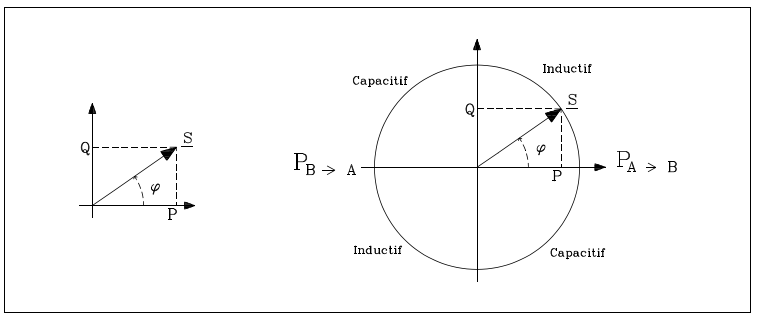
\includegraphics[scale=0.4]{ch1/image4.png}
		\captionof{figure}{ }
		\end{center}	
		
		\subsubsection{Puissance réactive}
		Dans l'expression $P = VI \cos\varphi = \Re(\underline{S})$, on définit la 
		\textbf{puissance réactive} :
		\begin{equation}
		Q = VI\sin\varphi = \Im(\underline{S})
		\end{equation}
		tel que $\underline{S} = P+jQ$.\\
		Si $P>0, Q>0$ si $\varphi>0$ c'est à dire que la charge est inductive.\\
		Si $P>0, Q<0$ si $\varphi<0$ c'est à dire que la charge est capacitive.\\
			
		La puissance réactive ne correspond à aucun travail effectif et est une 
		notion difficile à saisir. Retenons juste que sa circulation amène des 
		pertes et des chutes de tension. Cette puissance n'apparaît que si la 
		charge est réactive, c'est-à-dire peut stocker de l'énergie\footnote{Voir 
		1.2-14 du syllabus pour une image intuitive}.
		
\section{Caractéristiques d'un système polyphasé}
	\subsection{Modes de couplage des circuits polyphasés}
	Soit $m$ sources électrique indépendantes $S_1, S_2,\dots,S_m$ dont les tensions 
	ont la même valeur efficace et sont déphasé de $2\pi/m$ : système $m-$phasé 
	équilibre d'ordre direct :
	\begin{equation}
	\underline{E_i} = E_{1} \langle -(i-1)\frac{2\pi}{m}
	\end{equation}
	\textsc{Convention :} la phase 2 est située en arrière de la phase 1 et la 
	phase 3 en arrière de la phase 2 (en arrière signifie "[...] dans le temps").\\
	
	Voici un schéma de principe pour un tel système. Chacun des enroulements d'
	induit est raccordé par deux fils, il faudrait donc $2m$ conducteurs. Il existe 
	deux moyens d'économiser le métal conducteur :
	
		\subsubsection{a. Couplage en étoile avec fil neutre}
		L'idée est d'utiliser un conducteur de retour commun à tous les circuits 
		en réunissant les extrémités. On appelle $O$, le fil neutre parcouru par 
		la somme des courants débités par toutes les sources. Nécessitant $m+1$ 
		fil de ligne, il s'agit du couplage \textit{étoilé avec fil neutre}.\\
		
		La \textbf{tension simple} (ou de \textbf{phase}) d'un conducteur est 
		la différence de potentiel entre le conducteur et le neutre. Par 
		exemple : $\underline{V}_1 = \underline{V}_1-\underline{V}_0$. La 
		\textbf{tension composée} (ou \textbf{entre phases}) est la différence 
		de potentiel entre deux conducteurs. Par exemple : $\underline{U}_{12} = 
		\underline{V}_2-\underline{V}_1$.
		
		
		\subsubsection{b. Couplage en étoile sans fil neutre}
		Si toutes les impédances sont identiques, le circuit est équilibre et 
		la somme des courants de ligne est nulle : $\sum_{i=1}^m i_i=0$. Comme 
		le neutre n'est plus parcouru, on peut le supprimer. Le point $N'$, 
		neutre, possède le même potentiel que le point $N$ par symétrie : $N$ 
		est un point neutre artificiel. Cette installation comporte $m$ fils.\\
		
		Spoil : si les charges sont déséquilibrée on peut conserver ce montage 
		mais la tension de $N' \neq N$.Cherchons maintenant les relations liant 
		tension et phase.\\
		Soit $\underline{V}_1, \underline{V}_2$ les tensions mesurées entre 
		neutre de phase consécutives 1 et 2. Par symétries, elle sont égales 
		en tension efficace mais déphasées de $2\pi/m$ radians. Si $\underline{
		V_1}$ est la référence :
		\begin{equation}
		\begin{array}{ll}
		\underline{V_1} &= V\angle 0\\
		\underline{V_2} &= V\angle -\frac{2\pi}{m}
		\end{array}
		\end{equation}
		Le phaseur de la tension mesurée entre les phases 1 et 2 s'écrit
		\begin{equation}
		\underline{U}_{12} = \underline{V_2}-\underline{V_1}
		\end{equation}
		On voit que\footnote{??} 
		\begin{equation}
		\begin{array}{ll}
		\underline{U}_{12} &= 2\underline{V}_1\sin \frac{\pi}{m}e^{-j\left(
		\frac{\pi}{m}+\frac{\pi}{2}\right)}\\
		U_{12} &= 2V_1\sin\frac{\pi}{m}
		\end{array}
		\end{equation}
		
		La puissance transportée par une ligne équilibrée vaudra alors 
		\begin{equation}
		P = \Re(m \underline{V}_1\underline{I_1}^* = mV_1I_1\cos\varphi
		\end{equation}
		
		Si le point neutre n'est pas accessible, la seule tension mesurable 
		est $U_{12}$. En remplaçant dans $P$, la valeur $V_1$ tirée de 
		$U_{12}$ :
		\begin{equation}
		P = \frac{m}{2\sin\frac{\pi}{m}}U_{12}I_1\cos\varphi
		\end{equation}
		\textbf{Attention :} $\varphi$ est le déphasage entre tension simple 
		et courant et rien d'autre!
		
		
		\subsubsection{c. Couplage en polygone}
		On peut connecter la sortir de chacune des phases du générateur à 
		l'entrée de la phase contiguë et de même pour le récepteur. La somme 
		des f.e.m. alternatives équilibrées engendrée dans les phases du 
		générateurs étant nulles, on peut les connecter pour former un 
		\textbf{polygone fermé} (le courant ne circulera pas). On aura pour ça
		besoin de $m$ conducteurs distincts.\\
		
		Soit $\underline{I}_{12}$ et $\underline{I}_{23}$ les courants qui 
		circulent dans deux phases consécutives du générateur et $\underline{I}_
		2$, le courant traversant la ligne commune. Par Kirchoff :
		\begin{equation}
		\underline{I}_2 = \underline{I}_{12}-\underline{I}_{23}
		\end{equation}
		Or $\underline{I}_{12}$ et $\underline{I}_{23}$  sont égaux en 
		grandeur et entre eux se trouve un angle de $2\pi/m$. Par les 
		relations vectorielles :
		\begin{equation}
		\underline{I}_2 = \underline{I}_{12}\sin\frac{\pi}{m}e^{-j\left(\frac{
		\pi}{m}-\frac{\pi}{2}\right)}
		\end{equation} 
		
		
		\subsubsection{d. Puissance électrique transportée par une ligne}
		Cette puissance s'exprime par 
		\begin{equation}
		P = \Re(m\underline{U}_{12}\underline{I}_{12}^* = mU_{12}I_{12}\cos
		\varphi = \frac{m}{2\sin\frac{\pi}{m}}U_{12}I_1\cos\varphi
		\end{equation}
		La puissance transmise est bien indépendante du mode de couplage du 
		générateur / récepteur.